\section{A Multitask Test}

% We create a massive multitask test to assess the aggregate knowledge and problem solving ability of a single model. \mantas{We need to start more high-level. Mention that our benchmark consists of multiple-choice questions.} The questions span $57$ subjects and were primarily collected from online sources of freely available practice questions. We indicate the level of difficulty of a subject with ``high school'', ``college'', or ``professional.'' \dan{note 57 is the number of atari games} For instance, professional subjects that we test include the Examination for Professional Practice in Psychology, the United States Medical Licensing Examination, the Certified Public Accountant exam, and the Bar exam for law. Because our suite of tests covers a diverse set of subjects, a model must be a well-rounded ``polymath'' to attain high performance. Our benchmark is therefore a challenging testbed that will also make it easier to systematically identify blindspots in machine learning systems.\collin{repetitive?}
% Unlike previous datasets that test general-purpose linguistic understanding [GLUE, SuperGLUE], or ``commonsense'' tasks trivial for humans, our benchmark assesses general-purpose understanding of subjects that can be expressed in text.

We create a massive multitask test consisting of multiple-choice questions from various branches of knowledge.
The test spans subjects in the humanities, social sciences, hard sciences, and other areas that are important for some people to learn. 
% topics humans care about and learn, we want humans to learn these, important that some (other) people have expertise in these subjects
There are $57$ tasks in total, 
which is also the number of Atari games \citep{Bellemare2013Atari}, 
all of which are listed in \Cref{app:fulllist}.
The questions in the dataset were manually collected by graduate and undergraduate students from freely available sources online. These include practice questions for tests such as the Graduate Record Examination and the United States Medical Licensing Examination. It also includes questions designed for undergraduate courses and questions designed for readers of Oxford University Press books. 
Some tasks cover a subject, like psychology, but at a specific level of difficulty, such as ``Elementary,'' ``High School,'' ``College,'' or ``Professional.''
For example, the ``Professional Psychology'' task draws on questions from freely available practice questions for the Examination for Professional Practice in Psychology, while the ``High School Psychology'' task has questions like those from Advanced Placement Psychology examinations.
%Our test enables researchers to pinpoint blindspots in pretrained models. 

We collected $15908$ questions in total, which we split into a few-shot development set, a validation set, and a test set. The few-shot development set has $5$ questions per subject, the validation set may be used for selecting hyperparameters and is made of $1540$ questions, and the test set has $14079$ questions. Each subject contains $100$ test examples at the minimum, which is longer than most exams designed to assess people.

\begin{figure}[t]
    \centering
    \vspace{-17pt}
    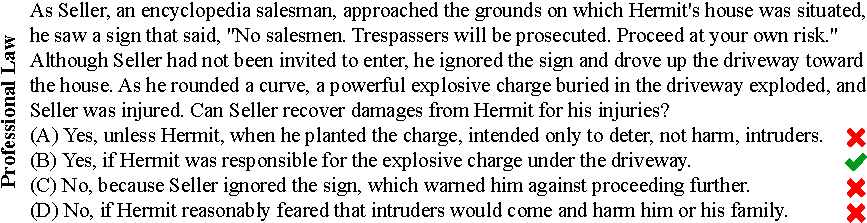
\includegraphics[width=\textwidth]{figures/law_figure.pdf}
    \caption{This task requires understanding detailed and dissonant scenarios, applying appropriate legal precedents, and choosing the correct explanation. The green checkmark is the ground truth.}
    \label{fig:law}
    \vspace{-17pt}
\end{figure}

Human-level accuracy on this test varies. Unspecialized humans from Amazon Mechanical Turk obtain $34.5\%$ accuracy on this test. Meanwhile, expert-level performance can be far higher. For example, real-world test-taker human accuracy at the 95th percentile is around $87\%$ for US Medical Licensing Examinations, and these questions make up our ``Professional Medicine'' task. If we take the 95th percentile human test-taker accuracy for exams that build up our test, and if we make an educated guess when such information is unavailable, we then estimate that expert-level accuracy is approximately $89.8\%$.

Since our test aggregates different subjects and several levels of difficulty, we measure more than straightforward commonsense or narrow \emph{linguistic} understanding. Instead, we measure arbitrary real-world \emph{text} understanding.
Since models are pretrained on the Internet, this enables us to test how well they can extract useful knowledge from massive corpora. Future models that use this test could be single models or a mixture of experts model.
To succeed at our test, future models should be well-rounded, possess extensive world knowledge, and develop expert-level problem solving ability.
These properties make the test likely to be an enduring and informative goalpost.
% this could be attained with a single model or a mixture of specialized expert models.

% The diversity of the test makes it 
%, and must be a well-rounded ``polymath.'' 
% want to test how well models can extract knowledge via pretraining

% the word "suite" is not used yet

% At the same time, we propose a methodological change to evaluate models more like how we evaluate humans. Most people do not prepare for exams by doing thousands of practice questions. Instead, they train by reading books on a particular topic. We make models take a similar approach by requiring that they answer questions in a zero-shot or few-shot setting, rather than by fine-tuning on thousands of practice questions. %This suggests that pretraining methods will need to become more efficient at extracting information from specialized texts before models can achieve high performance.
% This design choice makes it possible to test a very wide range of subjects since it means one does not need to collect massive training sets for every subject one wishes to evaluate. In the process, it also removes the possibility that models can rely on spurious cues [], which ensures that it provides an accurate estimate of actual performance.


% It would be infeasible to collect many thousands of practice questions for every subject for fine-tuning

% collected questions for $57$ subjects, including fields in STEM, the humanities, the social sciences, and more. To ensure standardization, we encode each of these in multiple choice questions with four options. These range in difficulty from an early high school level to an advanced professional level. We collected some questions from high school or college level course material, some from standardized exams like the Bar exam for law and the MCAT for medical school, and some from non-academic sources such as for pop culture trivia and global facts. In the rest of this section, we provide more details about the subjects included. Full details can be found in the appendix.
% 57. Massive multitask. Assess a single model. Mostly from freely available practice questions online. Professional exams like Bar, EPPP, USMLE, professional accounting. Diverse subjects, well-rounded. Indicate difficulty with high school, college, professional. Well-rounded since a single model; polymath. Prepare by reading books not solely by taking practice tests; extract from blob. Find blindspots. "Suite". general-purpose linguistic understanding vs general-purpose text understanding

\subsection{Humanities}
The humanities is a group of disciplines that make use of qualitative analysis and analytic methods rather than scientific empirical methods. Branches of the humanities include law, philosophy, history, and so on (\Cref{app:fulllist}). Mastering these subjects requires a variety of skills. For example, legal understanding requires knowledge of how to apply rules and standards to complex scenarios, and also provide answers with stipulations and explanations. We illustrate this in \Cref{fig:law}.
Legal understanding is also necessary for understanding and following rules and regulations, a necessary capability to constrain open-world machine learning models.
%understanding human approval and disapproval, which may make it an important component of value learning [ETHICS].
For philosophy, our questions cover concepts like logical fallacies, formal logic, and famous philosophical arguments. It also covers moral scenarios, including questions from the ETHICS dataset \citep{hendrycks2020ethicsdataset} that test a model's understanding of normative statements through predicting widespread moral intuitions about diverse everyday scenarios. Finally, our history questions cover a wide range of time periods and geographical locations, including prehistory and other advanced subjects.
%It even covers prehistory, which helps probe a model's knowledge of concepts rarely mentioned in everyday text.


% Law has Complex scenarios. Answer with explanation/Model human approval and disapproval/ Important for EU.
% Philosophy concepts like statements and fallacies. Detailed questions about seminal papers in philosophy. We probe the positions taken on the different sides of longstanding moral disputes, and we use commonsense morality question from ETHICS. Prehistory too; things that are rarely mentioned on reddit and everyday text.

% Subjects we include from the humanities include history, philosophy, and law. History includes prehistory, US history, European history, and world history. Philosophy includes formal logic, logical fallacies, and world religions. Law includes international law, jurisprudence, and professional law.
% An example of a question from professional law comes from the Bar exam, and is shown in \Cref{fig:law}. \collin{TODO: also talk about how important law is, and perhaps how it is connected to ethics.}

\subsection{Social Science}
Social science includes branches of knowledge that examine human behavior and society. Subject areas include economics, sociology, politics, geography, psychology, and so on. See \Cref{fig:socsci} for an example question. Our economics questions include microeconomics, macroeconomics, and econometrics, and cover different types of problems, including questions that require a mixture of world knowledge, qualitative reasoning, or quantitative reasoning.
We also include important but more esoteric topics such as security studies in order to test the boundaries of what is experienced and learned during pretraining.
Social science also includes psychology, a field that may be especially important for attaining a nuanced understanding of humans.

% What is social science about/Humans and society and use empirical methods.
% Basic economics about different economic models.
% Also more esoteric topics such as security studies.
% Psychology EPPP; nuanced answers about complicated subject, humans.

\begin{figure}[t]
    \centering
    \vspace{-20pt}
    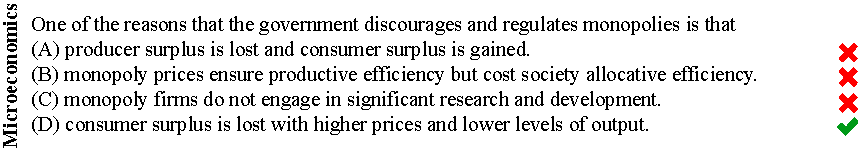
\includegraphics[width=\textwidth]{figures/social_sciences_thin.pdf}
    \caption{Examples from the Microeconomics task. %and Security Studies social science tasks.
    \looseness=-1}
    \label{fig:socsci}
    % \vspace{-10pt}
\end{figure}

\begin{figure}[t]
    \centering
    % \vspace{-20pt}
    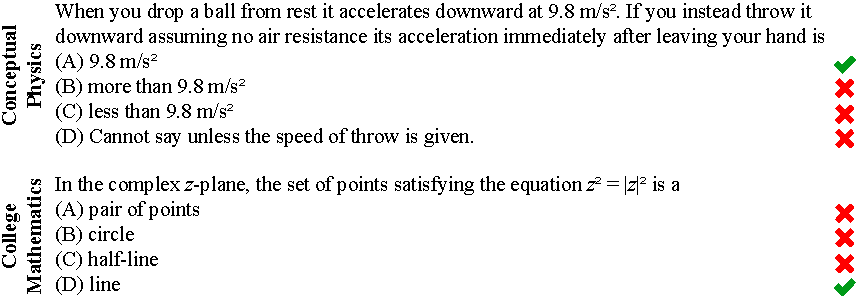
\includegraphics[width=\textwidth]{figures/stem.pdf}
    \caption{Examples from the Conceptual Physics and College Mathematics STEM tasks.
    \looseness=-1}
    \label{fig:stem}
    \vspace{-10pt}
\end{figure}

\subsection{Science, Technology, Engineering, and Mathematics (STEM)}
STEM subjects include physics, computer science, mathematics, and more. Two examples are shown in \Cref{fig:stem}. Conceptual physics tests understanding of simple physics principles and may be thought of as a harder version of the physical commonsense benchmark Physical IQA \citep{bisk2019physicaliqa}. We also test mathematical problem solving ability at various levels of difficulty, from the elementary to the college level.
College mathematics questions, like those found on the GRE mathematics subject test, often require chains of reasoning and abstract knowledge. To encode mathematics expressions, we use LaTeX or symbols such as * and \^{} for multiplication and exponentiation respectively. STEM subjects require knowledge of empirical methods, fluid intelligence, and procedural knowledge.


% % STEM covers subjects in science, technology, engineering, and mathematics. 
% % These subjects require more mathematics and sequential problem solving than other fields.
% This includes topics like physics, machine learning, and mathematics.
% By emphasizing problem solving, STEM questions tend to test procedural knowledge (i.e. knowledge about how to perform a task) more than the humanities and social sciences, which tend to test more descriptive knowledge (i.e. knowledge that a given statement is true). 

% To encode questions with math in text, we use a combination of LaTeX and symbols like * and \^{} for multiplication and exponentiation respectively. 
% We show example questions from conceptual physics and abstract algebra in \Cref{fig:stem}. Conceptual physics may be thought of as a harder version of Physical IQA [], a dataset that tests physical common sense.

% mathematics at various levels of difficulty.

% \collin{Show a problem/subject area that requires more sequential problem solving than this abstract algebra problem, then describe that.}
% Abstract algebra is a more specialized subject but requires less notation to express on average than other subjects in mathematics. 
% We will show later that STEM subjects tend to be the hardest subjects for existing models. 

% What is STEM about? Higher emphasis on mathematics and sequential problem solving and procedural knowledge.
% Conceptual Physics/Maths Figure
% Maths: sequential decision making/crystalized intelligence/problem solving/reasoning. Abstract algebra might be relatively easy since most problems are expressed with fewer symbols. We encode problems with LaTeX or symbols like \^.
% Conceptual Physics: PIQA. More symbolic option.
% We shall see that this area is hardest.

\subsection{Other}
There is a long tail of subjects that either do not neatly fit into any of the three preceding categories or for which there are not thousands of freely available questions. We put these subjects into Other.
This section includes the Professional Medicine task, which has difficult questions that require humans many years of study to master.
An example is depicted in \Cref{fig:other}.
This section also contains business topics like finance, accounting, and marketing, as well as knowledge of global facts. The latter includes statistics about poverty in different countries over time, which may be necessary for having an accurate model of the world internationally.
%and which could eventually be important for understanding large scale societal trends.
% Finally, we also assess topics like Fermi estimation and agriculture, for which for which there are not many questions with answers widely available.

% What is Other about? Long tail of concepts.
% Professional Medicine Figure
% Accounting and valuation.
% Global facts important for understanding the macrodynamics and forecasting.
% Long tail of concepts for which we did not find many hundreds of questions with answers like fermi estimation, computer literacy, and agriculture.

\begin{figure}[t]
    \centering
    \vspace{-15pt}
    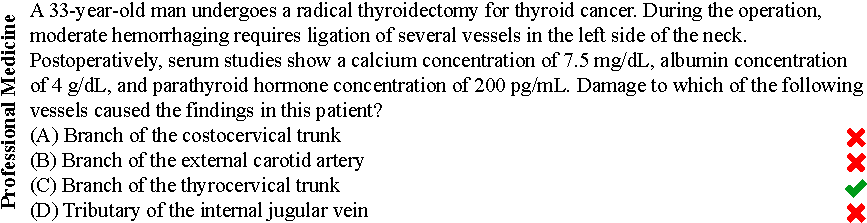
\includegraphics[width=\textwidth]{figures/medicine_figure.pdf}
    \caption{A question from the Professional Medicine task.% which is a simulated question from the United States Medical Licensing Examination.
    }
    \label{fig:other}
    \vspace{-15pt}
\end{figure}